%%%%%%%%%%%%%%%%%%%%%%%%%%%%%%%%%%%%%%%%%
% baposter Landscape Poster
% LaTeX Template
% Version 1.0 (11/06/13)
%
% baposter Class Created by:
% Brian Amberg (baposter@brian-amberg.de)
%
% This template has been downloaded from:
% http://www.LaTeXTemplates.com
%
% License:
% CC BY-NC-SA 3.0 (http://creativecommons.org/licenses/by-nc-sa/3.0/)
%
%%%%%%%%%%%%%%%%%%%%%%%%%%%%%%%%%%%%%%%%%

%----------------------------------------------------------------------------------------
%	PACKAGES AND OTHER DOCUMENT CONFIGURATIONS
%----------------------------------------------------------------------------------------

\documentclass[a0paper,fontscale=0.22]{baposter} % Adjust the font scale/size here

\usepackage{graphicx} % Required for including images
\graphicspath{{figures/}} % Directory in which figures are stored

\usepackage{amsmath} % For typesetting math
\usepackage{amssymb} % Adds new symbols to be used in math mode

\usepackage{booktabs} % Top and bottom rules for tables
\usepackage{enumitem} % Used to reduce itemize/enumerate spacing
\usepackage{palatino} % Use the Palatino font
\usepackage[font=small,labelfont=bf]{caption} % Required for specifying captions to tables and figures
%\usepackage{hyperref}

\usepackage{multicol} % Required for multiple columns
\setlength{\columnsep}{1.5em} % Slightly increase the space between columns
\setlength{\columnseprule}{0mm} % No horizontal rule between columns

\usepackage{tikz} % Required for flow chart
\usetikzlibrary{shapes,arrows} % Tikz libraries required for the flow chart in the template

\newcommand{\compresslist}{ % Define a command to reduce spacing within itemize/enumerate environments, this is used right after \begin{itemize} or \begin{enumerate}
\setlength{\itemsep}{1pt}
\setlength{\parskip}{0pt}
\setlength{\parsep}{0pt}
}

\definecolor{lightblue}{rgb}{0.145,0.6666,1} % Defines the color used for content box headers

\begin{document}

\begin{poster}
{
headerborder=closed, % Adds a border around the header of content boxes
colspacing=1em, % Column spacing
bgColorOne=white, % Background color for the gradient on the left side of the poster
bgColorTwo=white, % Background color for the gradient on the right side of the poster
borderColor=lightblue, % Border color
headerColorOne=black, % Background color for the header in the content boxes (left side)
headerColorTwo=lightblue, % Background color for the header in the content boxes (right side)
headerFontColor=white, % Text color for the header text in the content boxes
boxColorOne=white, % Background color of the content boxes
textborder=roundedleft, % Format of the border around content boxes, can be: none, bars, coils, triangles, rectangle, rounded, roundedsmall, roundedright or faded
eyecatcher=true, % Set to false for ignoring the left logo in the title and move the title left
headerheight=0.2\textheight, % Height of the header
headershape=roundedright, % Specify the rounded corner in the content box headers, can be: rectangle, small-rounded, roundedright, roundedleft or rounded
headerfont=\Large\bf\textsc, % Large, bold and sans serif font in the headers of content boxes
%textfont={\setlength{\parindent}{1.5em}}, % Uncomment for paragraph indentation
linewidth=2pt % Width of the border lines around content boxes
}
%----------------------------------------------------------------------------------------
%	TITLE SECTION 
%----------------------------------------------------------------------------------------
%
{
\includegraphics[height=6em]{julogo}} % First university/lab logo on the left
{\bf\textsc{EvoloPy: An Open-Source Nature-Inspired Optimization Framework in Python}\vspace{0.5em}} % Poster title
{\textsc{\{ H. Faris, I. Aljarah S. Mirjalili, P. A. Castillo and JJ Merelo \} \hspace{12pt}  U. of Granada}} % Author names and institution
{
\includegraphics[height=6em]{granadalogo}} % Second university/lab logo on the right
%----------------------------------------------------------------------------------------
%	INTRODUCTION
%----------------------------------------------------------------------------------------


\headerbox{Why Python?}{name=method,column=0}{ % This block's bottom aligns with the bottom of the conclusion block
\large
\begin{itemize}\compresslist
\item  Python: general purpose, clear and simple syntax. 

\item  Popular in scientific computing.

\item  Cross-platform. 

\item  Minimal setup.

\item  Uses modular and object based programming.
\end{itemize}
%----------------------------------------------------------------------------------------
%	MATERIALS AND METHODS
%----------------------------------------------------------------------------------------



%\begin{itemize}\compresslist
%\item Curabitur pellentesque dignissim
%\item Eu facilisis est tempus quis
%\item Duis porta consequat lorem
%\item Eu facilisis est tempus quis
%\end{itemize}


}

\headerbox{Framework Overview}{name=introduction,column=1,row=0}{


EvoloPy provides a set of classical and recent nature-inspired metaheuristic optimizers with an easy-to-use interface. 

Main components of the framework are: 

\begin{itemize}\compresslist
\item The {\tt Optimizer}. 

\item The metaheuristic {\tt Algorithms}:

\item Benchmark functions and problem definitions.

\item Result analysis.

\vspace{1em}

\end{itemize}}


\headerbox{Design issues}{name=conclusion,column=2,row=0}{

\begin{itemize}\compresslist

\item Using {\tt NumPy} extensively: simple and compact syntax for
  vector operations.

\item Populations as 2-dimensional arrays;  individuals as
  1-dimensional arrays (\texttt{ndarray} from \texttt{Numpy}).

\item 11 classes: \begin{itemize} 
    \item 8 for optimizers,
    \item 3 for optimization.
\end{itemize}

\end{itemize}

}



%----------------------------------------------------------------------------------------
%	RESULTS 1
%----------------------------------------------------------------------------------------

\headerbox{Comparison with Matlab}{name=results,column=0,span=3,row=0,below=introduction}{

\LARGE
NumPy rocks.
%------------------------------------------------

\begin{multicols}{2}
\vspace{1em}

\begin{center}
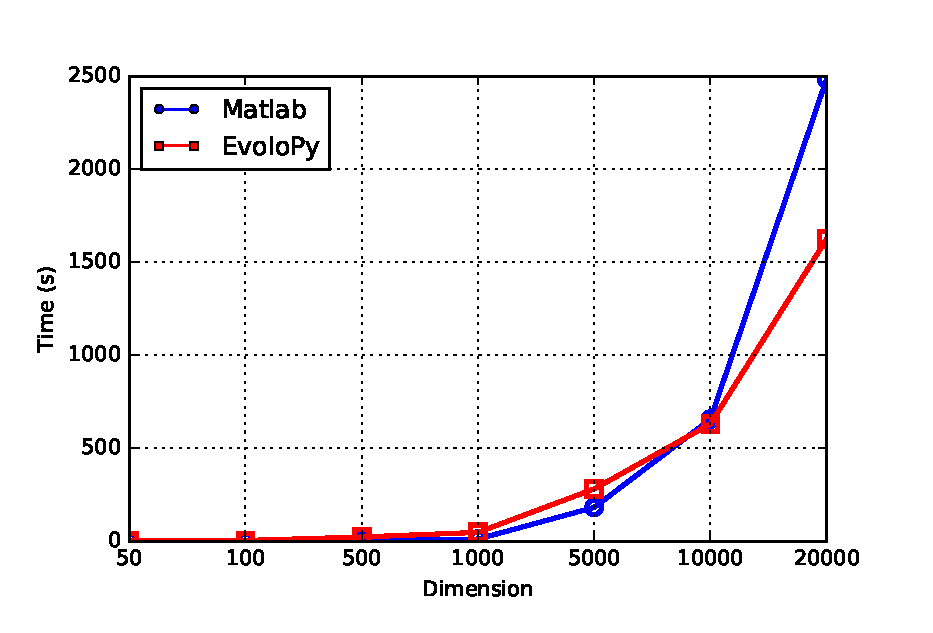
\includegraphics[width=0.95\linewidth]{PSO}
\captionof{figure}{PSO}
\label{fig:pso}
\end{center}


\begin{center}
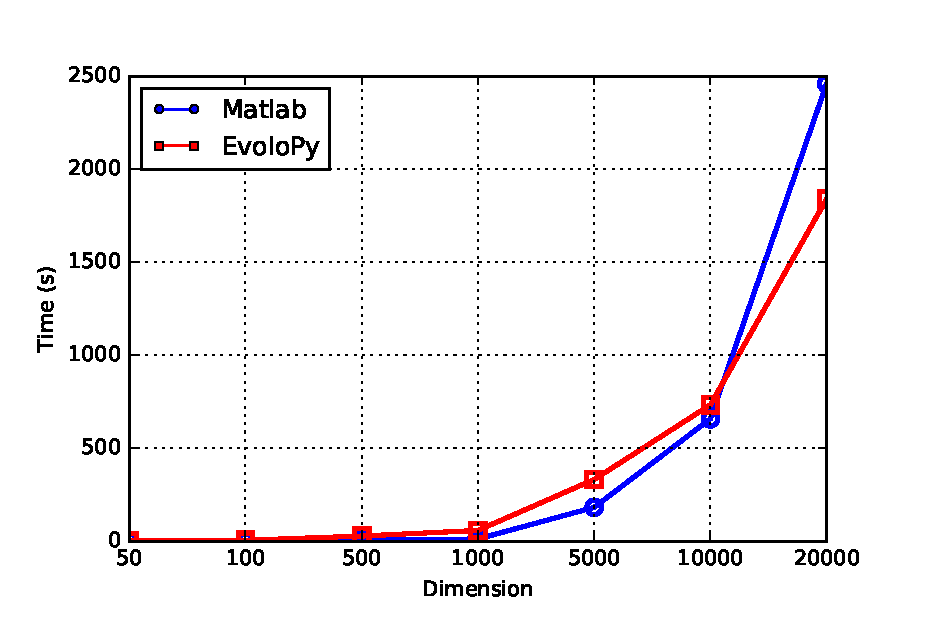
\includegraphics[width=0.95\linewidth]{GWO}
\captionof{figure}{GWO}
\label{fig:gwo}
\end{center}





\end{multicols}
}

%----------------------------------------------------------------------------------------



%----------------------------------------------------------------------------------------
%	REFERENCES
%----------------------------------------------------------------------------------------

\headerbox{Contact}{name=references,column=0,below=results}{

KASIT, The University of Jordan
\{hossam.faris, i.aljarah\}@ju.edu.jo

ETSIIT-CITIC, University of Granada, Granada, Spain
\{pedro, jmerelo\}@geneura.urg.es

}


%----------------------------------------------------------------------------------------
%	CONCLUSIONS
%----------------------------------------------------------------------------------------

\headerbox{Highlights}{name=objectives,column=1,span=2,row=3,below=results}{
\Large

\begin{enumerate}\compresslist
\item {\tt EvoloPy} is open source and cross-platform. 
\item Makes easier using metaheuristic algorithms for their own
  problems or creating new ones.
\item Free software!
\end{enumerate}

\centerline
{\tt github.com/7ossam81/EvoloPy}

\vspace{0.3em} % When there are two boxes, some whitespace may need to be added if the one on the right has more content
}

\end{poster}

\end{document}